\chapter{Communication}
To get the data from the computer, that is used for the GOT system, to the Arduino on the vehicle, there is needed a communication system. This will be done through two Xbee radio modules. The communication setup for the Xbee modules will be explain in this chapter.

\subsection{Wireless communication with Xbee}

%Notes:
%We use UDP, no connections

%OSI
%The physical layer is the Xbee
%The data link layer is halfway done in the code, where the package is split up in bytes. The adressing is done on the XBee and in the serial port libeary 
%The network layer may not be used here as we just transmit 360 degree
%The transport layer is the setup of how the package is setup
%The rest of the layers is not used.


\subsection{Transport Layer}
To understand the what each byte contains, when they are send from the transmitter to receiver, there is made a protocol for the transport layer. The use of a protocol for the transport layer will make sure that each end of the communication system understand how each package of bytes is build up.

The main object for the communication system is to send the data from the GOT system to the Arduino. To make sure that the data is received correctly and that none disturbances, like bit shifting, have changed the data, there will also be send error handling parts with the data. The error handling will not repair damaged packages, but throw them away instead. This is because the sampling time for the GOT system is so low (10 hertz), that the vehicle can go on, even if one or two package gets thrown away. Also if the system try to repair the package, the package had to be resend or have a repair part included, which will make the packages bigger.

To make the protocol, each part of the package have to be converted into bit arrays.

\subsubsection{Data}
The data from the GOT system is considered as the three coordinates (X, Y and Z) that the GOT system have measure for the vehicle. Each of these coordinates can have a value from -9000 to 9000 (See \secref{GoTDescription}). To contain number of this size, there is needed a 15 bit signed integer. 14 bit is used for the magnitude of the number, which can go up to 16385 ($2^{14}-1$). The last bit is used to indicate if the number is positive or negative, called signed bit. The signed bit will be placed at the end of the 15 bit integer. As both the Arduino and the computer, for the GOT system, use big endians, this will also be apply to the protocol. This means that the bit with highest value will be next to the sign bit and the bit with the lowest value at the start of the bit array. This will give the bit array seen on \tableref{CoorSetup}.

\begin{table}[H]
\centering
\begin{tabular}{|>{\centering\arraybackslash}m{0.5cm}|>{\centering\arraybackslash}m{0.5cm}|>{\centering\arraybackslash}m{0.5cm}|>{\centering\arraybackslash}m{0.5cm}|>{\centering\arraybackslash}m{0.5cm}|>{\centering\arraybackslash}m{0.5cm}|>{\centering\arraybackslash}m{0.5cm}|>{\centering\arraybackslash}m{0.5cm}|>{\centering\arraybackslash}m{0.5cm}|>{\centering\arraybackslash}m{0.5cm}|>{\centering\arraybackslash}m{0.5cm}|>{\centering\arraybackslash}m{0.5cm}|>{\centering\arraybackslash}m{0.5cm}|>{\centering\arraybackslash}m{0.5cm}|>{\centering\arraybackslash}m{0.65cm}|}
\multicolumn{15}{c}{15 bits} \\
\hline
$2^0$ & $2^1$ & $2^2$ & $2^3$ & $2^4$ & $2^5$ & $2^6$ & $2^7$ & $2^8$ & $2^9$ & $2^{10}$ & $2^{11}$ & $2^{12}$ & $2^{13}$ & $+/-$ \\
\hline
\end{tabular}
\caption{Setup for the bit array, that contains one of the coordinate values.}
\label{CoorSetup}
\end{table}

The representation of the integer is called signed magnitude. Another representation that could be used is ones' complement. Here the number is inverted, if the signed bit is true. But for easier the implementation into the code for the GOT system, signed magnitude is used. This is easier because the code will first check if the number is positive or negative. If negative, the sign bit is set and the number is multiply by minus one, to get the magnitude. Then the magnitude will then be converted into the bit array. When converting it back, there is only needed to multiply the magnitude by minus one, if the signed bit is true.

\subsubsection{Header}
The header of the protocol contains the information about who have to receive the package (destination) and the length of the package (length). These header is used, to make communication in bigger networks easier to handle.

With the destination, the transmitter can say which receiver have to catch the package. This way the transmitter can send to multiple receiver, in the case where there multiple vehicles. This is used on the receiver, to filter out all the packages, that was not send to it, but it still catches it. In this project the vehicle will get the destination ID 0000 0001. The length of the destination byte is set to one byte, so the destination can be read by itself, when it is received.

There could also be applied a source to the header, but as it is only the computer that is sending and the vehicle do not need to know where the coordinates come from, even if there are more computers, as long as the data is marked with the destination for it self. If there was used a resend method, in case of damaged packages, the source would have been needed, to know where to ask for a resend. But as there is not, the source will not be implemented in this protocol.

The information about the length is used by the receiver, to see how many bit there is in the package and in this way, know how much it still needs to receive, before it have the whole package. As each package contains the same parts in this system and these parts do not get shorter or longer, only have different values, the length will be the same for each package. The size of the bit array, that contains the length, set to 7 bit, as this can contain up to 127. This number is considered high enough, as the package is set to be as small as possible.

With the header the transmitter can send to specific receivers and the receiver can receive packages specified for it and know the length of the whole package.

\subsubsection{Checksum}
To make sure that the package data is received correctly, there is added some error handling to the protocol. One of these is a checksum. The way the checksum is calculated, is by splitting the header and data up in parts of equal size and then adding these parts together. Then the summed bit array is inverted and this bit array is the checksum. 

As there is 60 bit in the header and the data combined (15 per coordinate, 8 for the destination and 7 for the length), these will be split up into three part of 20 bit and will give a checksum on 20 bit. Combined, the header, data and checksum will be 80 bit, which is equal to 10 byte, which means there will not be needed any filler bit.

\begin{table}[H]
\centering
\begin{tabular}{c c c c c c c c c c c}
   & Bit array  &     & Decimal &     & Bit 0-3 & Bit 4-7 & Bit 8-11 & Bit 12-15 & Bit 16-19 & Bit 20 \\
\hline
a) & Part 1     & $=$ & 123008  & $=$ & 0000 & 0001 & 0000 & 0111 & 1000 & \\
b) & Part 2     & $=$ & 351365  & $=$ & 1010 & 0001 & 0011 & 1010 & 1010 & \\
c) & Part 3     & $=$ & 729671  & $=$ & 1110 & 0010 & 0100 & 0100 & 1101 & \\
d) & Part 1+2+3 & $=$ & 1204044 & $=$ & 0011 & 0010 & 1111 & 1010 & 0100 & 1 \\
e) & Add carry  & $=$ & 155469  & $=$ & 1011 & 0010 & 1111 & 1010 & 0100 & \\
f) & Checksum   & $=$ & 893106  & $=$ & 0100 & 1101 & 0000 & 0101 & 1011 & \\
g) & Check      & $=$ & 1048575 & $=$ & 1111 & 1111 & 1111 & 1111 & 1111 & \\
\end{tabular}
\caption{Example on how to calculated the checksum. The parts contains the header, where the length is set to 96 and the coordinates 4259, 7511 and -6418. The binary number is writing up in big endians.}
\label{ChecksumExp}
\end{table}

In \tableref{ChecksumExp} there is a example on the calculation for the checksum. The three parts contains the header and data and these are added together (seen on line d). This gives a carry, that is added on in the start of the number (seen on line e). The new number is then inverted and this is then the checksum (seen on line f).

The way to control for error with the checksum, is to add the checksum together with the three 20 bit parts and add the carry on, if there are any. If the outcome of this addition is a 20 bit part, where all bits is true, the package is correctly received. If not, the control will say that there is a error in the package and it will be thrown away. The reason for the error can be a bit shift in one of the parts, that there are bytes that have switch placed or some data have not be received. 

A flaw with this control with the checksum, is that if a error goes out with another error, this can not be detected. This can happen when the system add the three parts and the checksum together. An example, is if the first bit in part one is true and the first bit in part two is false. If both of these bit is bit shifted, so the bit from part one is equal false and true for the bit in part two, this error will not be detected by the control with the checksum. The chances for this is very small, as the changes have to go exactly out with each other. And by only having 4 parts of 20 bits, the chances for this to happen is smaller than if the checksum was set to, for example to 10 bit and therefore addition have to happen with 7 parts of 10 bit. This will give more bits, there have the same value, so there is a higher chance, for the changing in the part to go out with each other. This is the reason for using a bigger checksum, even if it takes more place.

\subsubsection{Start and end byte}
As the GOT system send a package each time it makes a measurement of the coordinates, there can come a queue of package at the Arduino, if it does not read fast enough. This can give the problem that the system can not tell the package from each other. This can be avoided by adding a start byte at the start of the package and a end byte at the end. 

When the system wants to find the start of the package, it will search for the start byte. When it have found this byte, it will read the header, data and checksum and then look for the end byte. If the end byte is not there, it means that the package was not received correctly and is thrown away. If the end byte is there, the system will take the whole package and make error handling on it. 

The start byte will be set to 0000 1111. This is chosen, so that the start byte do not have the same value as one of the other bytes, that is in the header, so these not will be misunderstand as the start byte. To have the start and end byte as different as possible, as the end byte will come just before the next start byte, the end byte is the inverted version of the start byte, which is 1111 0000.

With the data, header, checksum, start and end byte, a package will look like the illustration on \tableref{PackageLook}

\begin{table}[H]
\centering
\begin{tabular}{|c|c|>{\centering\arraybackslash}m{0.3cm}|>{\centering\arraybackslash}m{0.3cm}|>{\centering\arraybackslash}m{0.3cm}|>{\centering\arraybackslash}m{0.3cm}|>{\centering\arraybackslash}m{0.3cm}|>{\centering\arraybackslash}m{0.3cm}|>{\centering\arraybackslash}m{0.3cm}|>{\centering\arraybackslash}m{0.3cm}|>{\centering\arraybackslash}m{0.3cm}|>{\centering\arraybackslash}m{0.3cm}|>{\centering\arraybackslash}m{0.3cm}|>{\centering\arraybackslash}m{0.3cm}|>{\centering\arraybackslash}m{0.3cm}|>{\centering\arraybackslash}m{0.3cm}|>{\centering\arraybackslash}m{0.3cm}|>{\centering\arraybackslash}m{0.3cm}|}
\hline
\multicolumn{2}{|c|}{Offsets} & \multicolumn{8}{c}{Byte 1} & \multicolumn{8}{|c|}{Byte 2} \\
\hline
\multicolumn{1}{|c}{Byte} & \multicolumn{1}{|c|}{Bit} & 0 & 1 & 2 & 3 & 4 & 5 & 6 & 7 & 8 & 9 & 10 & 11 & 12 & 13 & 14 & 15 \\
\hline
0 & 0 & \multicolumn{8}{c}{Start byte} & \multicolumn{8}{|c|}{Destination} \\
\hline
2 & 16 & \multicolumn{7}{c}{Length} & \multicolumn{9}{|c|}{X coordinate} \\
\hline
4 & 32 & \multicolumn{6}{c}{X coordinate} & \multicolumn{10}{|c|}{Y coordinate} \\
\hline
6 & 48 & \multicolumn{5}{c}{Y coordinate} & \multicolumn{11}{|c|}{Z coordinate} \\
\hline
8 & 64 & \multicolumn{4}{c}{Z coordinate} & \multicolumn{12}{|c|}{Checksum} \\
\hline
10 & 80 & \multicolumn{8}{c}{Checksum} & \multicolumn{8}{|c|}{End byte} \\
\hline
\end{tabular}
\caption{Illustration of a package, that will be send from the transmitter to the receiver.}
\label{PackageLook}
\end{table}

This give a package length on 96 bits (12 bytes). As the GOT system have a sampling frequency on 10 hertz and each sampling give out 12 byte, the transfer speed for the Xbee have to be greater than 120 byte per second. 

\subsubsection{Error handling}
As there is a chance that the package is getting damaged under the way from the transmitter to the receiver, there is used some error handling, to check the packages for error and throw the damage packages away. One of these is the checksum, which is explained further up in this section. Besides the checksum, the start and end byte is used to see if the number of byte received is right, according to the length in the header.

But as with the checksum, where there was a flaw, if there are more errors and these cancel each other out in the control with the checksum, there is a flaw in the way the error handling for receiving packages. The receiving process can be seen on \figref{FlowReceiver}.

\begin{figure}[H]
\centering
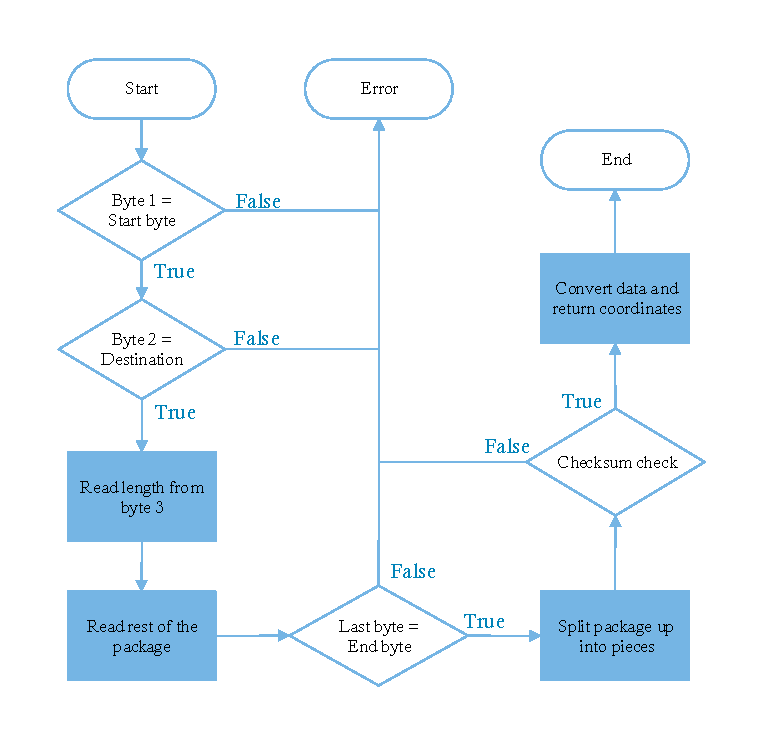
\includegraphics[scale=0.7]{figures/FlowReceiver.pdf}
\caption{Flow chart over the error handling in the receiver part.}
\label{FlowReceiver}
\end{figure}

If the package is transmitted correctly, the 1st byte will be the start byte, the 2nd byte will be the destination ID of the receiver. The 3rd byte will contain 7 bit for the length and 1 bit for the first coordinate. If the length is correct, it will be 96, which is 12 byte. The last byte, the 12th one, is the end byte. Then if these condition is all correct, the receiver will make a control with the checksum. If that one is also correct, the system will convert the data and return the coordinates to the rest of the system.

If there is an error, then all the bytes, that have been read will be thrown away. This is because that the bytes is taken from the buffer, that the receiving Xbee have and can not be put back in at the same place, after it have been taken out. So if the start byte and destination is correct, but the end byte is not, the whole package is thrown away and there will be looking for a new start byte. If the start byte is not correct, then only that byte will thrown away. The reason for using the method, is that the system only want to work with whole packages, so it searching for a whole package, by checking for the start byte, the header and then the end byte. So if the first is not equal to the start byte, it will never become a complete package. Therefore is the bytes already thrown away, before a whole package have been read.

By doing this, even if the receiver by fault start in the middle of a package, the system will just throw away the bad package, until it finds the start byte. A problem that comes with this feature, is that the start byte is only on a byte long and a byte in the data and checksum part can have the same value as it. If the receiver then by fault begin to look after the start byte in these part and find a byte equal to the start byte, it can become a problem. The problem will first happen, if the byte afterwards is equal to the receivers destination ID and the byte after that, first seven bits is equal to 96. If this is the case, the receiver will think that is have found the start byte and the header and will read the next 9 byte. An example on a situation where this problem happens can be seen on \tableref{errorPro}.

\begin{table}[H]
\centering
\begin{tabular}{c | m{0.1cm} m{0.1cm} m{0.1cm} m{0.1cm} m{0.1cm} m{0.1cm} m{0.1cm} m{0.1cm} | c | m{0.1cm} m{0.1cm} m{0.1cm} m{0.1cm} m{0.1cm} m{0.1cm} m{0.1cm} m{0.1cm} | l }
\multicolumn{9}{c}{Normal reading} & \multicolumn{9}{c}{Displaced reading} &  \\
\cline{2-9} \cline{11-18}
1st byte & 0 & 0 & 0 & 0 & 1 & 1 & 1 & 1 & 5th byte & 0 & 0 & 0 & 0 & 1 & 1 & 1 & 1 & $\leftarrow$ Start byte \\
\cline{2-9} \cline{11-18}
2nd byte & 0 & 0 & 0 & 0 & 0 & 0 & 0 & 1 & 6th byte & 0 & 0 & 0 & 0 & 0 & 0 & 0 & 1 & $\leftarrow$ Destination \\
\cline{2-9} \cline{11-18}
3rd byte & 0 & 0 & 0 & 0 & 0 & 1 & 1 & 0 & 7th byte & 0 & 0 & 0 & 0 & 0 & 1 & 1 & 0 & $\leftarrow$ Length (First seven bit)\\
\cline{2-9} \cline{11-18}
4th byte & 1 & 1 & 1 & 1 & 0 & 0 & 0 & 0 & 8th byte & 0 & 1 & 1 & 1 & 0 & 0 & 1 & 1 & \\
\cline{2-9} \cline{11-18}
5th byte & 0 & 0 & 0 & 0 & 1 & 1 & 1 & 1 & 9th byte & 1 & 0 & 0 & 1 & 1 & 0 & 1 & 1 & \\
\cline{2-9} \cline{11-18}
6th byte & 0 & 0 & 0 & 0 & 0 & 0 & 0 & 1 & 10th byte & 1 & 0 & 0 & 0 & 0 & 1 & 0 & 0 & \\
\cline{2-9} \cline{11-18}
7th byte & 0 & 0 & 0 & 0 & 0 & 1 & 1 & 0 & 11th byte & 0 & 0 & 1 & 1 & 0 & 1 & 1 & 1 & \\
\cline{2-9} \cline{11-18}
8th byte & 0 & 1 & 1 & 1 & 0 & 0 & 1 & 1 & 12th byte & 1 & 1 & 1 & 1 & 0 & 0 & 0 & 0 & \\
\cline{2-9} \cline{11-18}
9th byte & 1 & 0 & 0 & 1 & 1 & 0 & 1 & 1 & 1st byte & 0 & 0 & 0 & 0 & 1 & 1 & 1 & 1 & \\
\cline{2-9} \cline{11-18}
10th byte & 1 & 0 & 0 & 0 & 0 & 1 & 0 & 0 & 2nd byte & 0 & 0 & 0 & 0 & 0 & 0 & 0 & 1 & \\
\cline{2-9} \cline{11-18}
11th byte & 0 & 0 & 1 & 1 & 0 & 1 & 1 & 1 & 3rd byte & 0 & 0 & 0 & 0 & 0 & 1 & 1 & 0 & \\
\cline{2-9} \cline{11-18}
12th byte & 1 & 1 & 1 & 1 & 0 & 0 & 0 & 0 & 4th byte & 1 & 1 & 1 & 1 & 0 & 0 & 0 & 0 & $\leftarrow$ End byte\\
\cline{2-9} \cline{11-18}
\end{tabular}
\caption{Example of a normal reading of a package and a displaced reading of a package. The package contains the coordinates (-8222, 515, -3699). For the displaced reading, after the first package, there comes another package, that is equal to the first one.}
\label{errorPro}
\end{table}

For the example on \tableref{errorPro}, the 5th to 7th byte is equal to the start byte and the header. So if the system is looking after the start byte and find the 5th byte, before it finds the next 1st byte, it will begin to look for the header. In this case it will find it and as the 12th byte, which is in the next package, is equal to the end byte, the system thinks it have found a whole package. But as there also the control with the checksum, the package will not go through. The checksum, in this case, will not be the original checksum for the package, but another part of the package. As this checksum is not calculated to fit, the chance for the check goes through is so small that it will not be considerer to happen. 

But even if the wrong package is being stop by the control with the checksum, the 12 bytes still have been read and therefore have to be thrown. This will happen no matter if the end byte is correct or not, just as long as the system finds the start byte and the header. And in these 12 bytes, the next real start byte is also thrown away. In worst case scenario, the next three byte, after the ones that got thrown away, is equal to the start byte and header again, the same scenario will repeat it self and will go on, onto the three byte no longer equals the start byte and header.

These scenarios about beginning to read a package in the middle of a package is not that common, as there is needed for three bytes to be precisely alike the start byte and the header (The last bit in the last byte is from the x coordinate, so is not needed to be the same). Even if the data and checksum parts is 8 bytes long together, the chance is small and the system have to first to not recognize the real start byte and header. Even if both things happens, as the coordinate will chance for each package, because of the vehicle moving, the chance for it to happens more times in a row is so small, that it will not be considered. And as the system do not have a problem with missing one package, this flaw in the error handling will not considered a problem.


%Insert tail